% Copyright 2011-2012 David Hadka.  All Rights Reserved.
%
% This file is part of the MOEA Framework User Manual.
%
% Permission is granted to copy, distribute and/or modify this document under
% the terms of the GNU Free Documentation License, Version 1.3 or any later
% version published by the Free Software Foundation; with the Invariant Section
% being the section entitled "Preface", no Front-Cover Texts, and no Back-Cover
% Texts.  A copy of the license is included in the section entitled "GNU Free
% Documentation License".

\chapter{Introduction}

The MOEA Framework is a free and open source Java library for developing and experimenting with multiobjective evolutionary algorithms (MOEAs) and other general-purpose optimization algorithms.  A number of algorithms are provided out-of-the-box, including NSGA-II, $\epsilon$-MOEA, GDE3 and MOEA/D.  In addition, the MOEA Framework provides the tools necessary to rapidly design, develop, execute and statistically test optimization algorithms.

This user manual is divided into the following three parts:
\begin{description}
  \item [Beginner's Guide] - Provides an introduction to the MOEA Framework for new users.  Topics discussed include installation instructions, walking through some introductory examples, and solving user-specified problems.
  \item [Advanced Guide] - Introduces features provided by the MOEA Framework intended for academic researchers and other advanced users.  Topics include performing large-scale experimentation, statistically comparing algorithms, and advanced configuration options.
  \item [Developer's Guide] - Intended for software developers, this part details guidelines for contributing to the MOEA Framework.  Topics covered include the development of new optimization algorithms, software coding guidelines and other policies for contributors.
\end{description}

\section{Key Features}

\begin{itemize}
  \item Fast, reliable implementations of many state-of-the-art multiobjective evolutionary algorithms
  \item Extensible with custom algorithms, problems and operators
  \item Modular design for constructing new optimization algorithms from existing components
  \item Permissive open source license
  \item Fully documented source code
  \item Over 1000 test cases to ensure validity
\end{itemize}

\section{Other Java Frameworks}

There exist a number of Java optimization framework developed over the years.  This section discusses the advantages and disadvantages of each framework.

\subsection{Watchmaker Framework}
\begin{wrapfigure}{l}{4cm}
  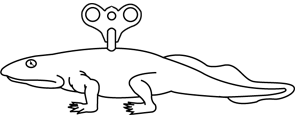
\includegraphics[width=4cm]{watchmaker.png}
\end{wrapfigure}
The Watchmaker Framework is one of the most popular open source Java libraries for single objective optimization.  Its design is non-invasive, allowing users to evolve objects of any type.  Most other framework (including the MOEA Framework) require the user to encode their objects using pre-defined decision variable types.  However, giving the users this freedom also increases the burden on the user to develop custom evolutionary operators for their objects.

\begin{quote}
\begin{description}
  \item[Homepage:] \webpage{http://watchmaker.uncommons.org}
  \item[License:] Apache License, Version 2.0
  \item[Advantages:]\ %force line break
    \begin{itemize}
      \item Very clean API
      \item Fully documented source code
      \item Flexible decision variable representation
      \item Large collection of interesting example problems (Mona Lisa, Sudoku, Biomorphs)
    \end{itemize}
  \item[Disadvantages:]\ %force line break
    \begin{itemize}
      \item Single objective only
      \item Much of the implementation burden is placed on the developer
      \item Infrequently updated (the last release, 0.7.1, was in January 2010)
    \end{itemize}
\end{description}
\end{quote}

\subsection{ECJ}
ECJ is a research-oriented Java library developed at the George Mason University�s Evolutionary Computation Laboratory.  Now in existence for nearly fourteen years, ECJ is a mature and stable framework.  It features a range of evolutionary paradigms, including both single and multiobjective optimization, master/save and island-model parallelization, coevolution, parsimony pressure techniques, with extensive support for genetic programming.  

\begin{quote}
\begin{description}
  \item[Homepage:] \webpage{http://cs.gmu.edu/~eclab/projects/ecj/}
  \item[License:] Academic Free License, Version 3.0
  \item[Advantages:]\ %force line break
    \begin{itemize}
      \item Quickly setup and execute simple EAs without touching any source code
      \item One of the most sophisticated open source libraries, particular in its support for various GP tree encodings
      \item Provides an extensive user manual, tutorials, and other developer tools
    \end{itemize}
  \item[Disadvantages:]\ %force line break
    \begin{itemize}
      \item Only minor support for multiobjective optimization
      \item Provides only outdated MOEAs (NSGA-II and SPEA2)
      \item Configuring EAs using ECJ�s configuration file can be cumbersome and error prone.  Testing shows that some errors introduced into the configuration file went undetected.
      \item Appears to lack any kind of automated testing or quality assurance
      \item Infrequent releases (the last release, version 20, was in October 2010)
    \end{itemize}
\end{description}
\end{quote}

\subsection{jMetal}
jMetal \index{jMetal} is a framework focused on the development, experimentation and study of metaheuristics.  As such, it includes the largest collection of metaheuristics of any framework discussed here.  If fact, the MOEA Framework incorporates the jMetal library for this very reason.  The jMetal authors have more recently started developing C++ and C\# versions of the jMetal library. 

\begin{quote}
\begin{description}
  \item[Homepage:] \webpage{http://jmetal.sourceforge.net}
  \item[License:] GNU Lesser General Public License, Version 3 or later
  \item[Advantages:]\ %force line break
    \begin{itemize}
      \item Focused on multiobjective optimization
      \item Implementations of 15 state-of-the-art MOEAs
      \item Provides an extensive user manual
    \end{itemize}
  \item[Disadvantages:]\ %force line break
    \begin{itemize}
      \item Not currently setup as a library; several places have hard-coded paths to resources located on the original developer�s computer
      \item Appears to lack any kind of automated testing or quality assurance
      \item Source code is not fully documented
      \item Infrequent releases (11 months between release 3.1 and 4.0)
    \end{itemize}
\end{description}
\end{quote}

\subsection{Opt4J}
\begin{wrapfigure}{l}{4cm}
  
\includegraphics[width=4cm]{opt4j.png}
\end{wrapfigure}
Opt4J provides perhaps the cleanest MOEA implementation.  It takes modularity to the extreme, using aspect-oriented programming to automatically stitch together program modules to form a complete, working optimization algorithm.  A helpful GUI for constructing experiments is also provided.

\begin{quote}
\begin{description}
  \item[Homepage:] \webpage{http://opt4j.sourceforge.net/}
  \item[License:] GNU Lesser General Public License, Version 3 or later
  \item[Advantages:]\ %force line break
    \begin{itemize}
      \item Focused on multiobjective optimization
      \item Uses aspect-oriented programming (AOP) via Google Guice to manage dependencies and wire all the components together
      \item Well documented source code
      \item Frequently updated
    \end{itemize}
  \item[Disadvantages:]\ %force line break
    \begin{itemize}
      \item Some unit tests, but they only cover a small fraction of the code base
      \item Only a limited number of MOEAs provided
    \end{itemize}
\end{description}
\end{quote}

%\subsection{JCLEC}
%
%\begin{quote}
%\begin{description}
%  \item[Homepage:] \webpage{http://jclec.sourceforge.net/}
%  \item[License:] GNU General Public License, Version 3 or later
%  \item[Advantages:]\ %force line break
%    \begin{itemize}
%      \item Extensive use of unit tests
%      \item Well documented source code
%    \end{itemize}
%  \item[Disadvantages:]\ %force line break
%    \begin{itemize}
%      \item GNU GPL license can not be mixed with other non-compatible licenses
%      \item Only minor support for multiobjective optimization
%      \item Provides only outdated MOEAs (NSGA-II and SPEA2)
%    \end{itemize}
%\end{description}
%\end{quote}
